\begin{center}
   {\colorbox{grey2}{
         \begin{minipage}[t]{0.9\textwidth}
         \subsubsection*{Scope}
     This Pirana Quick Guide explains how to prepare,  configure and work with a cluster over SSH, 
and how to subsequently work with Pirana to execute models on the cluster. 
         \end{minipage}
      }
   }
\end{center}

\subsubsection*{Preparation: SSH access}
In order to execute runs on a cluster from a local system with Pirana, SSH access
to the cluster from your local computer must be available. 
\begin{itemize}
\item For Windows, the easiest way to do this is to install
  \href{'http://www.chiark.greenend.org.uk/~sgtatham/putty/''}{Putty}. Make
  sure that you install the complete version of PuTTY, including the
  command line tool \emph{plink.exe}.
\item After installation, make sure Putty is available in the system
  path, or add the location of the Putty folder to the internal Pirana
  path via File $\rightarrow$ Settings $\rightarrow$ Software
  integration $\rightarrow$ 'Add this folder(s) to PATH at Pirana
  startup'.
\item On Linux and Mac OSX, ssh is most likely already installed.
\end{itemize}

\subsubsection*{Preparation: Mounting a cluster folder as local drive}
A remote folder on the cluster should be mounted as a local drive
letter (e.g. R:) on your system. There are several ways to do this,
some of which are described below. Please check with your system
administrator if you don't manage to mount the cluster as a local drive.
\begin{itemize}
\item If the cluster is running Samba, a drive letter may be mounted
  through My Computer $\rightarrow$ Extra $\rightarrow$ Network
  connections.
\item If only SSH (SFTP) access is available, software such as
  \href{'http://www.expandrive.com/''}{Expandrive} may be considered.
\end{itemize}



\subsubsection*{Configuring the cluster}
If the remote cluster folder can be mounted as drive letter on your
system, and you have installed putty, cluster access may now be
configured in Pirana.
\begin{itemize}
\item Access the settings menu via File $\rightarrow$ Settings
  $\rightarrow$ Clusters. A screen is obtained as depicted in Figure  \ref{fig:Fig1}.

\begin{figure}[h] \centering
    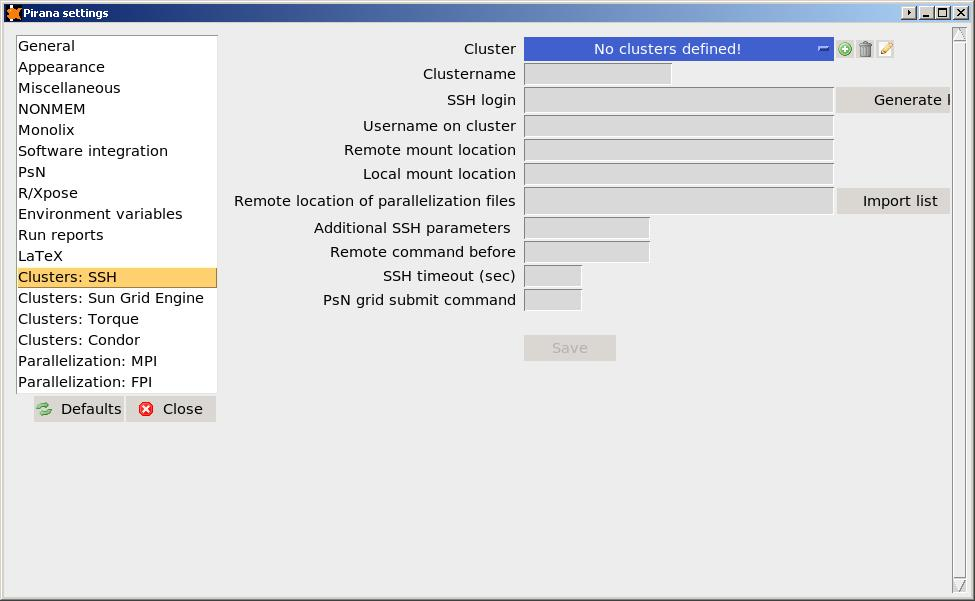
\includegraphics[scale=.4]{images/cluster_1.JPG}
    \caption{Cluster settings window\label{fig:Fig1}
}
\end{figure}

\item Select the \emph{\Large{+}} sign to add a new cluster. Some
  initial settings are pre-entered in the textboxes of the newly
  defined cluster (Figure  \ref{fig:Fig2}), but these have to be updated to match
  your cluster.

\begin{figure}[h] \centering
    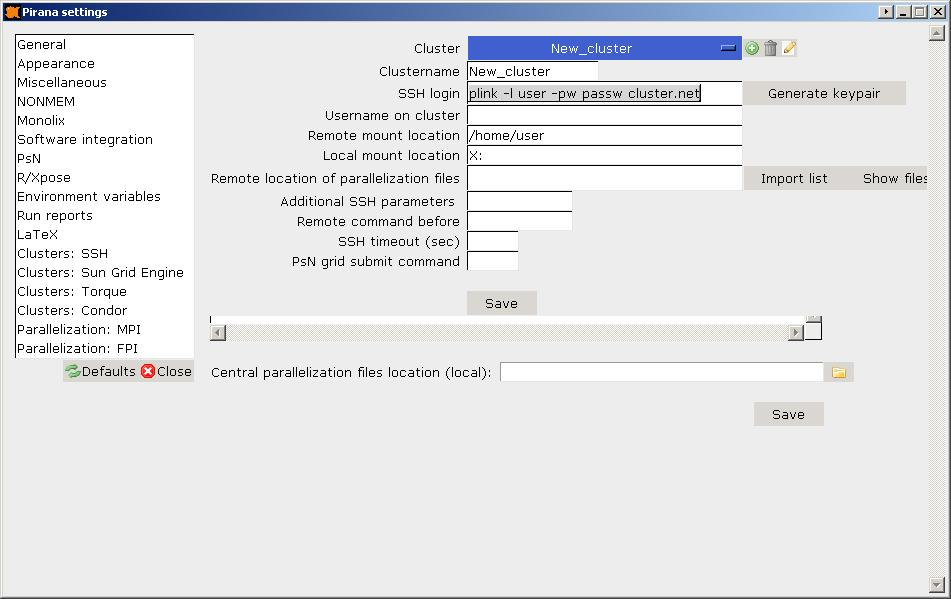
\includegraphics[scale=.4]{images/cluster_2.JPG}
    \caption{Pre-entered text after adding a new cluster\label{fig:Fig2}
}
\end{figure}

\item In the textbox \emph{Clustername}, define a name for the cluster
  (can be anything).
\item The textbox \emph{SSH login} should contain the command to
  connect to the cluster. If Putty is used, this command will start
  with \emph{plink}, followed by the user name, password and name or
  IP address of the cluster access node, e.g. 'plink -l myname -p
  mypassw pkpd.server.org'. Passwordless access using a RSA key is
  also possible.
\item The textbox \emph{Remote mount location} refers to a folder on
  the cluster which you have mounted as local drive.
\item The textbox \emph{Local mount location} should contain the
  drive-letter on the local system which corresponds with the remote
  cluster path defined in the previous textbox.
\item In the following textboxes, \emph{Additional SSH parameters},
  and \emph{Remote commands before} connecting to the cluster, and the
  \emph{PsN grid submit command} may be defined, but these are not
  required.
\item  An example of a fully configured cluster is depicted in Figure  \ref{fig:Fig3}.
\end{itemize}

\begin{figure}[h] \centering
    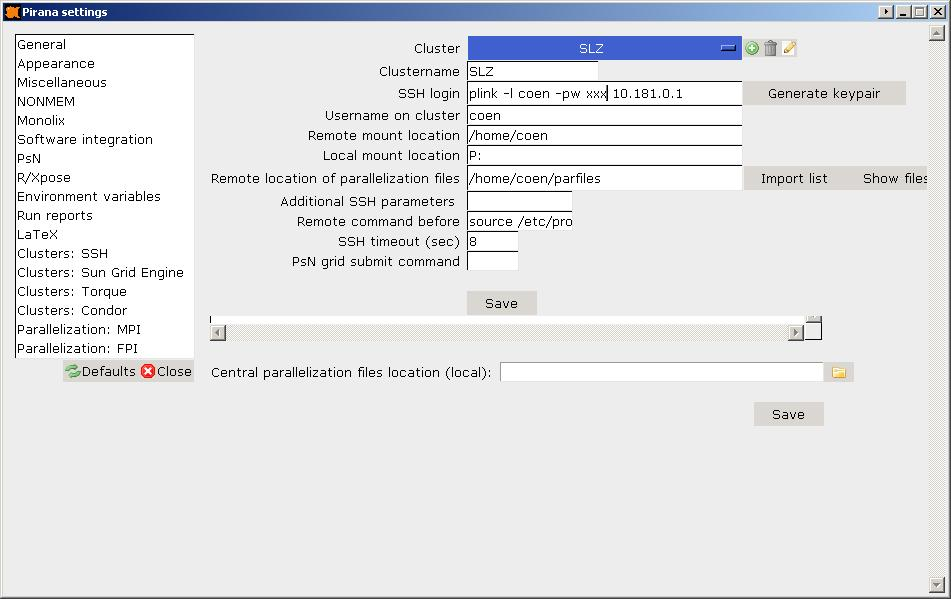
\includegraphics[scale=.4]{images/cluster_3b.JPG}
    \caption{Settings of a fully configured cluster\label{fig:Fig3}
}
\end{figure}

\subsubsection*{Working with the cluster}

  \begin{itemize}
  \item Any runs which are to be submitted to the cluster should be in
    a location on the drive which you specified the remote cluster
    mount location.
  \item A model can be run on the cluster via either \emph{nmfe} or
    \emph{PsN}, which are described separately below.
\end{itemize}

\subsubsection*{Submitting a run to the cluster via nmfe}
  \begin{itemize}
  \item When submitting a run via nmfe, after selecting a model and
    opening the 'nmfe'-run dialog, select a cluster to connect to
    (Figure  \ref{fig:Fig4}, blue quare).
  \item The option \emph{Submit to [..]} should be selected if the run is to be
    submitted to a job scheduler. (Figure  \ref{fig:Fig4}, green square). 
    Currently supported schedulers are Sun Grid Engine (SGE), Torque and Condor.
  \item Optionally, for NONMEM 7.2, parallalization files may be
    selected.
  \item Start the run.
\end{itemize}

\begin{figure}[h] \centering
    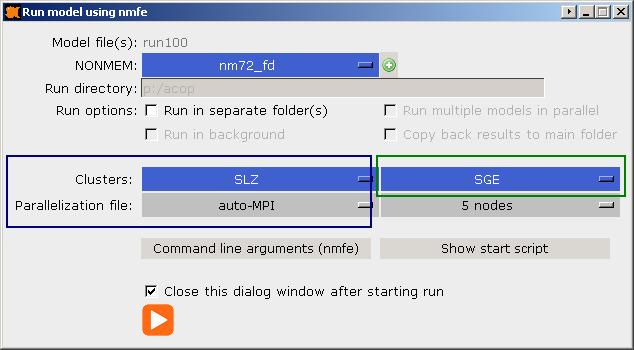
\includegraphics[scale=.4]{images/cluster_4.JPG}
    \caption{Defining cluster settings for a nmfe run\label{fig:Fig4}
}
\end{figure}

\pagebreak

\subsubsection*{Submitting a run to the cluster via PsN}
  \begin{itemize}
  \item Select a cluster for the PsN run (Figure 5, orange square).
  \item Add optional arguments to the PsN argument, such as
    \emph{-run\_on\_sge}, if the run is submitted to SGE (Figure  \ref{fig:Fig5},
    red square).
  \item Several PsN arguments are available for other job schedulers
    such as LSF (Figure  \ref{fig:Fig5}, blue square). Please note that
    the configuration of these job schedulers should be done in the
    psn.conf file on the cluster. Please refer to the PsN manual for
    more information about this.
  \item Start the run.
\end{itemize}

\begin{figure}[h] \centering
    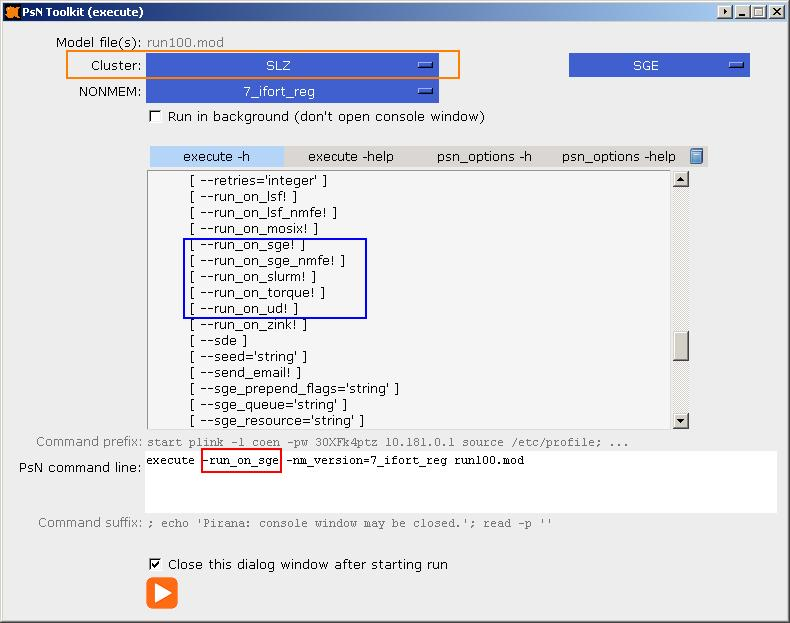
\includegraphics[scale=.4]{images/cluster_5.JPG}
    \caption{Defining cluster settings for a PsN run\label{fig:Fig5}
}
\end{figure}

\subsubsection*{Monitoring jobs on a SGE cluster}
  \begin{itemize}
  \item If SGE, Torque or Condor is used as job managment system, the queue may be
    monitored using the integrated monitor in Pirana.
  \item This feature may be accessed by clicking the SGE icon in the
    main Pirana interface (Figure \ref{fig:Fig2}, red square).
  \item In the interface that is opened, an overview will be presented
    of the jobs that are currently running, scheduled, or have
    recently been finished. Some information about available nodes in
    the SGE cluster can also be viewed.
  \item By right-clicking on a job, you can view more information
    about it, or kill it. Please note that not only NONMEM jobs are
    shown here, but any compute job (e.g. MATLAB).
\end{itemize}

\begin{figure}[h] \centering
    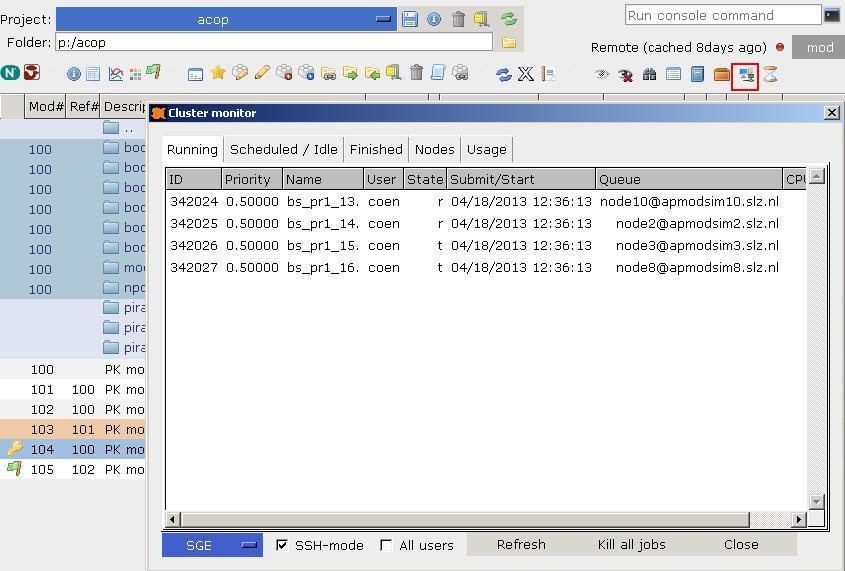
\includegraphics[scale=.4]{images/cluster_6.JPG}
    \caption{Cluster run window\label{fig:Fig6}
}
\end{figure}
